\documentclass[11pt]{article}
\usepackage[T1]{fontenc}
\usepackage[utf8]{inputenc}
\usepackage{graphicx}
\usepackage{minitoc}
\usepackage[french]{babel}
\usepackage[right=2.5cm, bottom=2.5cm,top=2.5cm, left=2.5cm]{geometry}
\title{\vspace{\fill} Cryptographie et sécurité \\ ~\textbf{IFT-606} \\~\\ Devoir 1 - Cryptographie et attaques}
\author{Amandine Fouillet - 14 130 638 ~\\ Frank Chassing - 14 153 710}
\date{\today \vspace{\fill}}

\begin{document}
\maketitle
\newpage \thispagestyle{empty}
\null
\newpage
\tableofcontents
\listoffigures
\newpage
\section{Wi-Fi}
\subsection{Fonctionnement des trois algorithmes de chiffrement}
\subsection{Points faibles et attaques possibles des trois algorithmes de chiffrement}
\subsection{Aircrack-ng}
\section{Chiffrement et signature}
\subsection{Génération d'une paire de clé RSA}
\begin{figure}[hbtp]
    \begin{minipage}[b]{0.4\linewidth}
        \centering 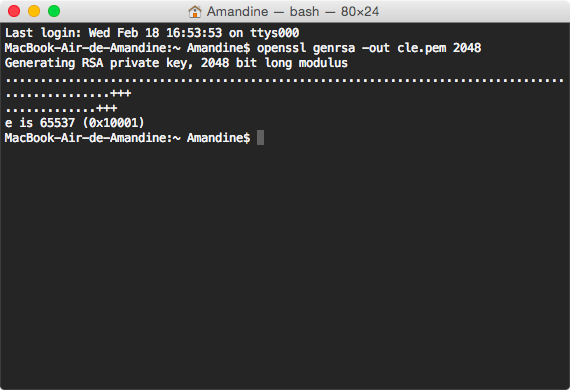
\includegraphics[scale=0.4]{q21.png}
        \caption{Génération de la paire}
                \label{fig:gen}
\label{fig:base}
    \end{minipage}\hfill
    \begin{minipage}[b]{0.48\linewidth}
        \centering 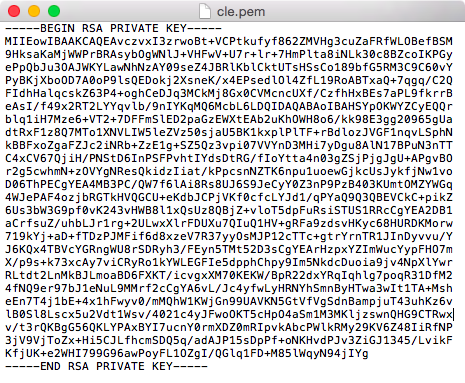
\includegraphics[scale=0.4]{q21b.png}
        \caption{Fichier obtenu}
         \label{fig:cle}
    \end{minipage}
\end{figure}

\subsection{Création d'un fichier contenant la partie publique de la clé RSA}
\subsection{Chiffrement de la partie privée générée}
\subsection{Chiffrement d'un message}
\subsection{Déchiffrement d'un message}
\subsection{Signature du fichier}
\section{Attaque décortiquée}

\end{document}